\subsection{演習}

Rust プレイグラウンドは、小規模のプログラムをテストし、新しいクレートとライブラリを試し、他のユーザーとコードを共有する場合に便利です。 この演習では、プレイグラウンドで小規模のプログラムをビルドして、この環境について理解を深めます。

\subsubsection{プレイグラウンドでコードを記述する}

まず、基本的なプログラムのコードを記述します。

\begin{enumerate}
\item Rust playground に接続します。

\item プレイグラウンド エディターで次のコードを入力します。

\begin{lstlisting}[numbers=none]
fn main(){println!(Welcome to Rust!);}
\end{lstlisting}

\item $[$Tools][Rustfmt] の順に選択し、コードを書式設定します。

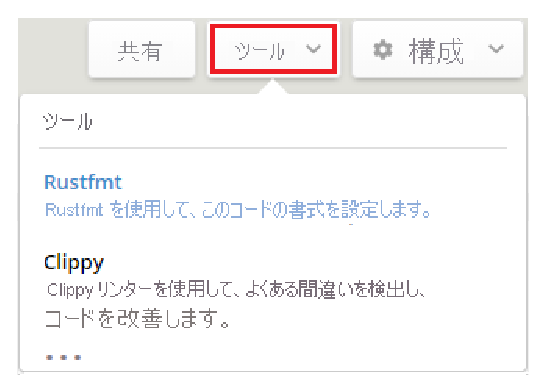
\includegraphics[width=10cm]{rust-playground-tools.eps}

このツールでは、公式の Rust スタイルを試用するようにコードを調整します。

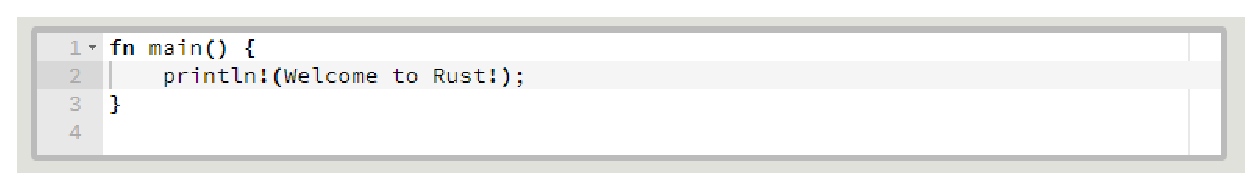
\includegraphics[width=14cm]{rust-playground-rustfmt.eps}

\item $[$Tools][Clippy] の順に選択して、コード内の誤りを確認します。 結果はエディターの下に表示されます。

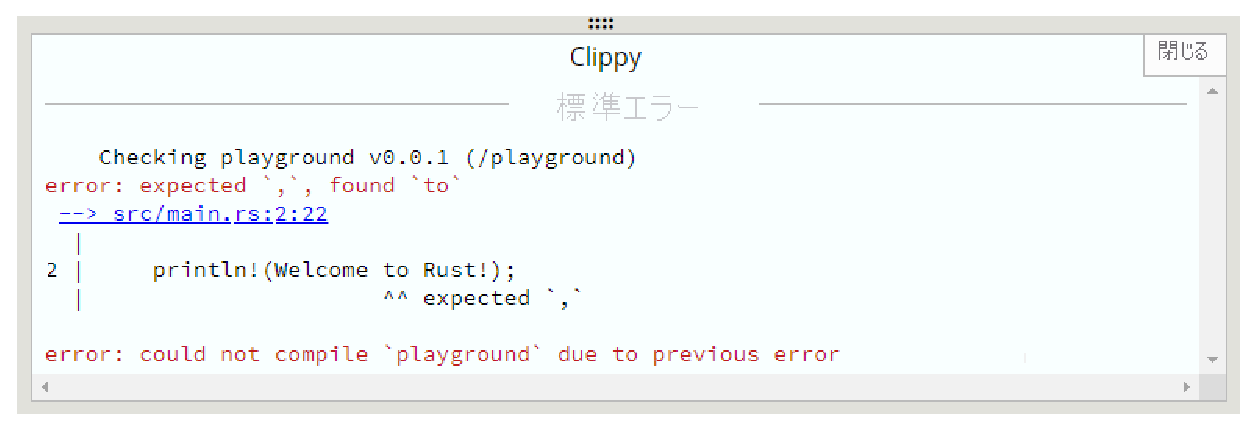
\includegraphics[width=14cm]{rust-playground-clippy.eps}

\item サンプル コードを修正するには、"Welcome to Rust!" というテキストの前後に引用符を追加します。

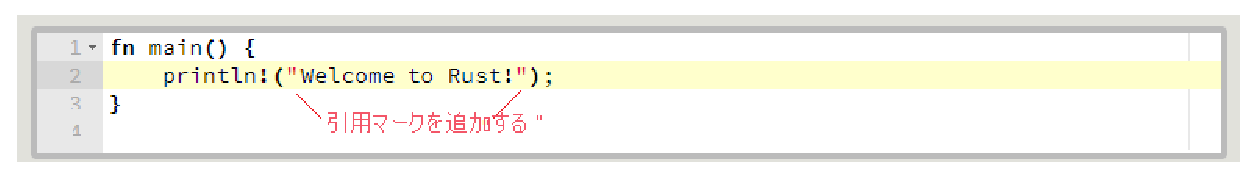
\includegraphics[width=14cm]{rust-playground-add-quotes.eps}

\end{enumerate}


\subsubsection{プレイグラウンドでコードをビルドして実行する}

次に、コードをコンパイルして、プログラムを実行します。

\begin{enumerate}
\item プレイグラウンドでコードをビルドして実行する方法を選択するには、UI の上部にある [Run] ドロップダウン メニューを開きます。

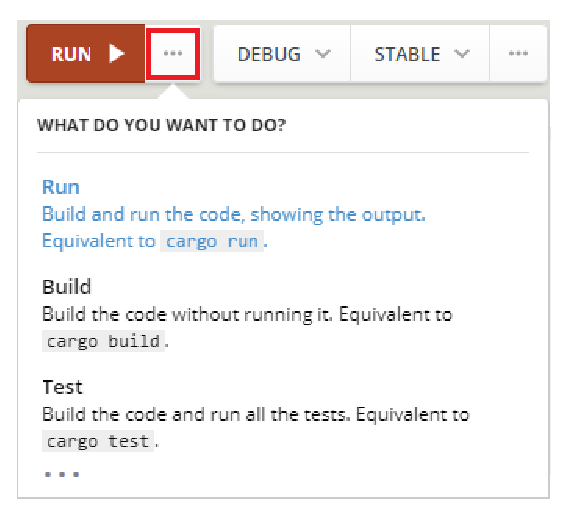
\includegraphics[width=10cm]{rust-playground-run.eps}

\item $[$Run] を選択して、サンプル プログラムをビルドして実行します。 プログラムの出力がエディターの下に表示されます。

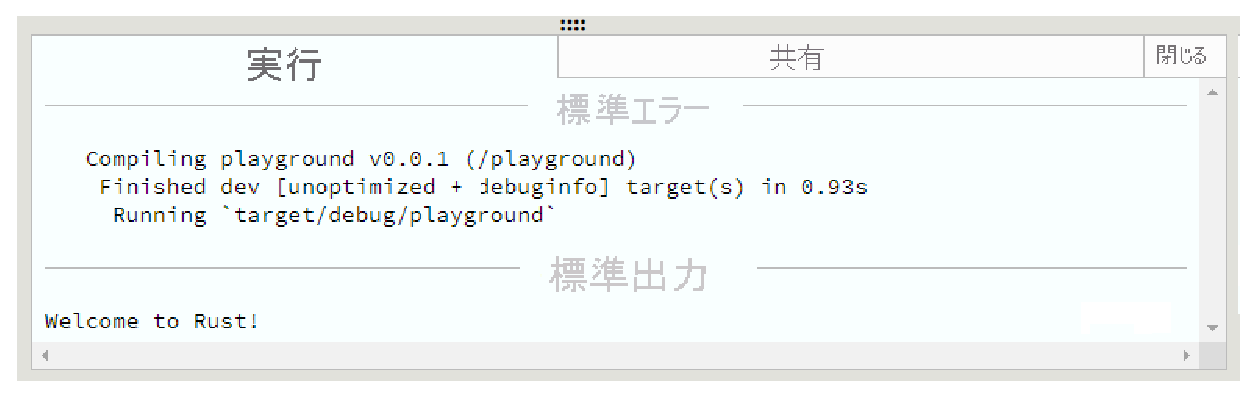
\includegraphics[width=14cm]{rust-playground-print.eps}

\end{enumerate}

\subsubsection{プレイグラウンドでコードを保存して共有する}

プレイグラウンドで作業するときに、コードはブラウザー ストレージに自動的に保存されます。 ブラウザー ウィンドウを閉じると、入力したコードが失われる場合があります。 コードを常に使用できるようにするために、共有可能な URL を作成できます。

\begin{enumerate}
\item ツール バーの [Share] 機能を選択して、プレイグラウンド内のコードの GitHub gist を作成します。

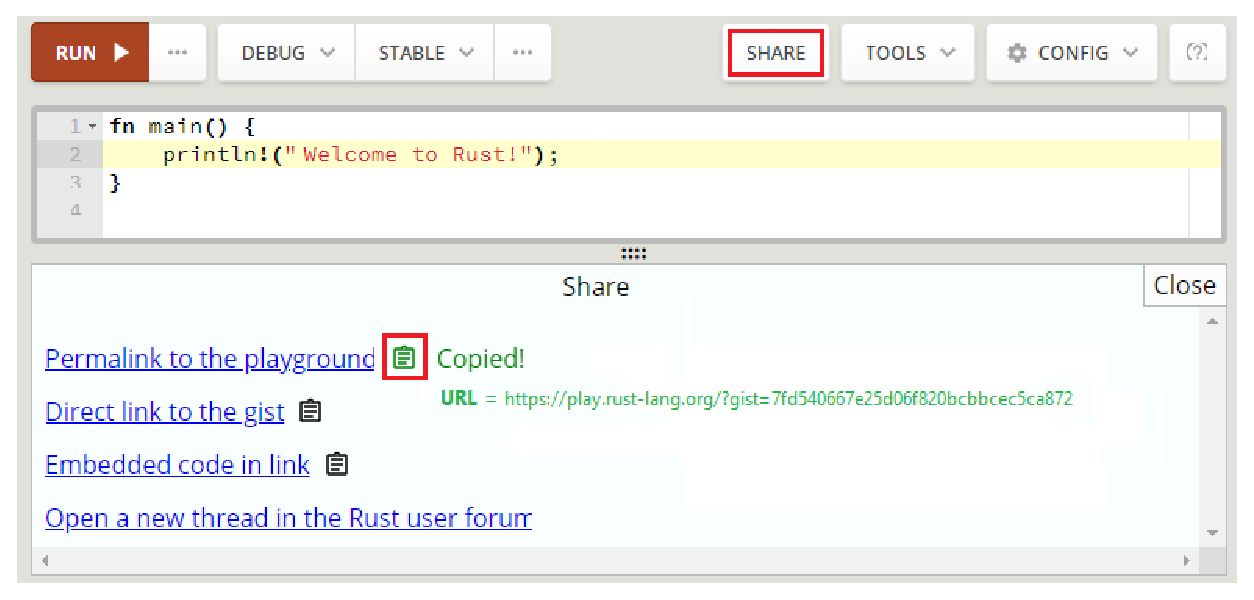
\includegraphics[width=14cm]{rust-playground-share.eps}

\item $[$Permalink to the playground] というテキストの横にある紙のアイコンを選択して、コードの共有可能 gist を取得します。
\end{enumerate}

これで、URL を保存して後でコードにアクセスするか、URL を共有して他の人がコードを確認できます。




